\documentclass{article}

% Language setting
% Replace `english' with e.g. `spanish' to change the document language
\usepackage[english]{babel}

% Set page size and margins
% Replace `letterpaper' with`a4paper' for UK/EU standard size
\usepackage[letterpaper,top=2cm,bottom=2cm,left=3cm,right=3cm,marginparwidth=1.75cm]{geometry}

% Useful packages
\usepackage{amsmath}
\usepackage{graphicx}
\usepackage[colorlinks=true, allcolors=blue]{hyperref}

\title{CPE301L: Lab 5}
\author{Joshua Knight, Nicky Victoriano}

\begin{document}
\maketitle
 
\section{Introduction}

In this lab, we are responsible for programming an Arduino to produce notes at different frequencies. Our keyboard input (A, B, C, D, E, F, G) will activate a timer that generates a square wave, creating the frequency that plays a note on a connected speaker.

\section{Results}

\subsection{Circuit}

To create the circuit, a buzzer was placed in the center of the breadboard. One side was wired to 'GND' on the Arduino Mega, and the other side was wired through a 100 $\Omega$ resistor and onto pin 12 as seen in Figure 1. 

\begin{figure}[h!]
\centering
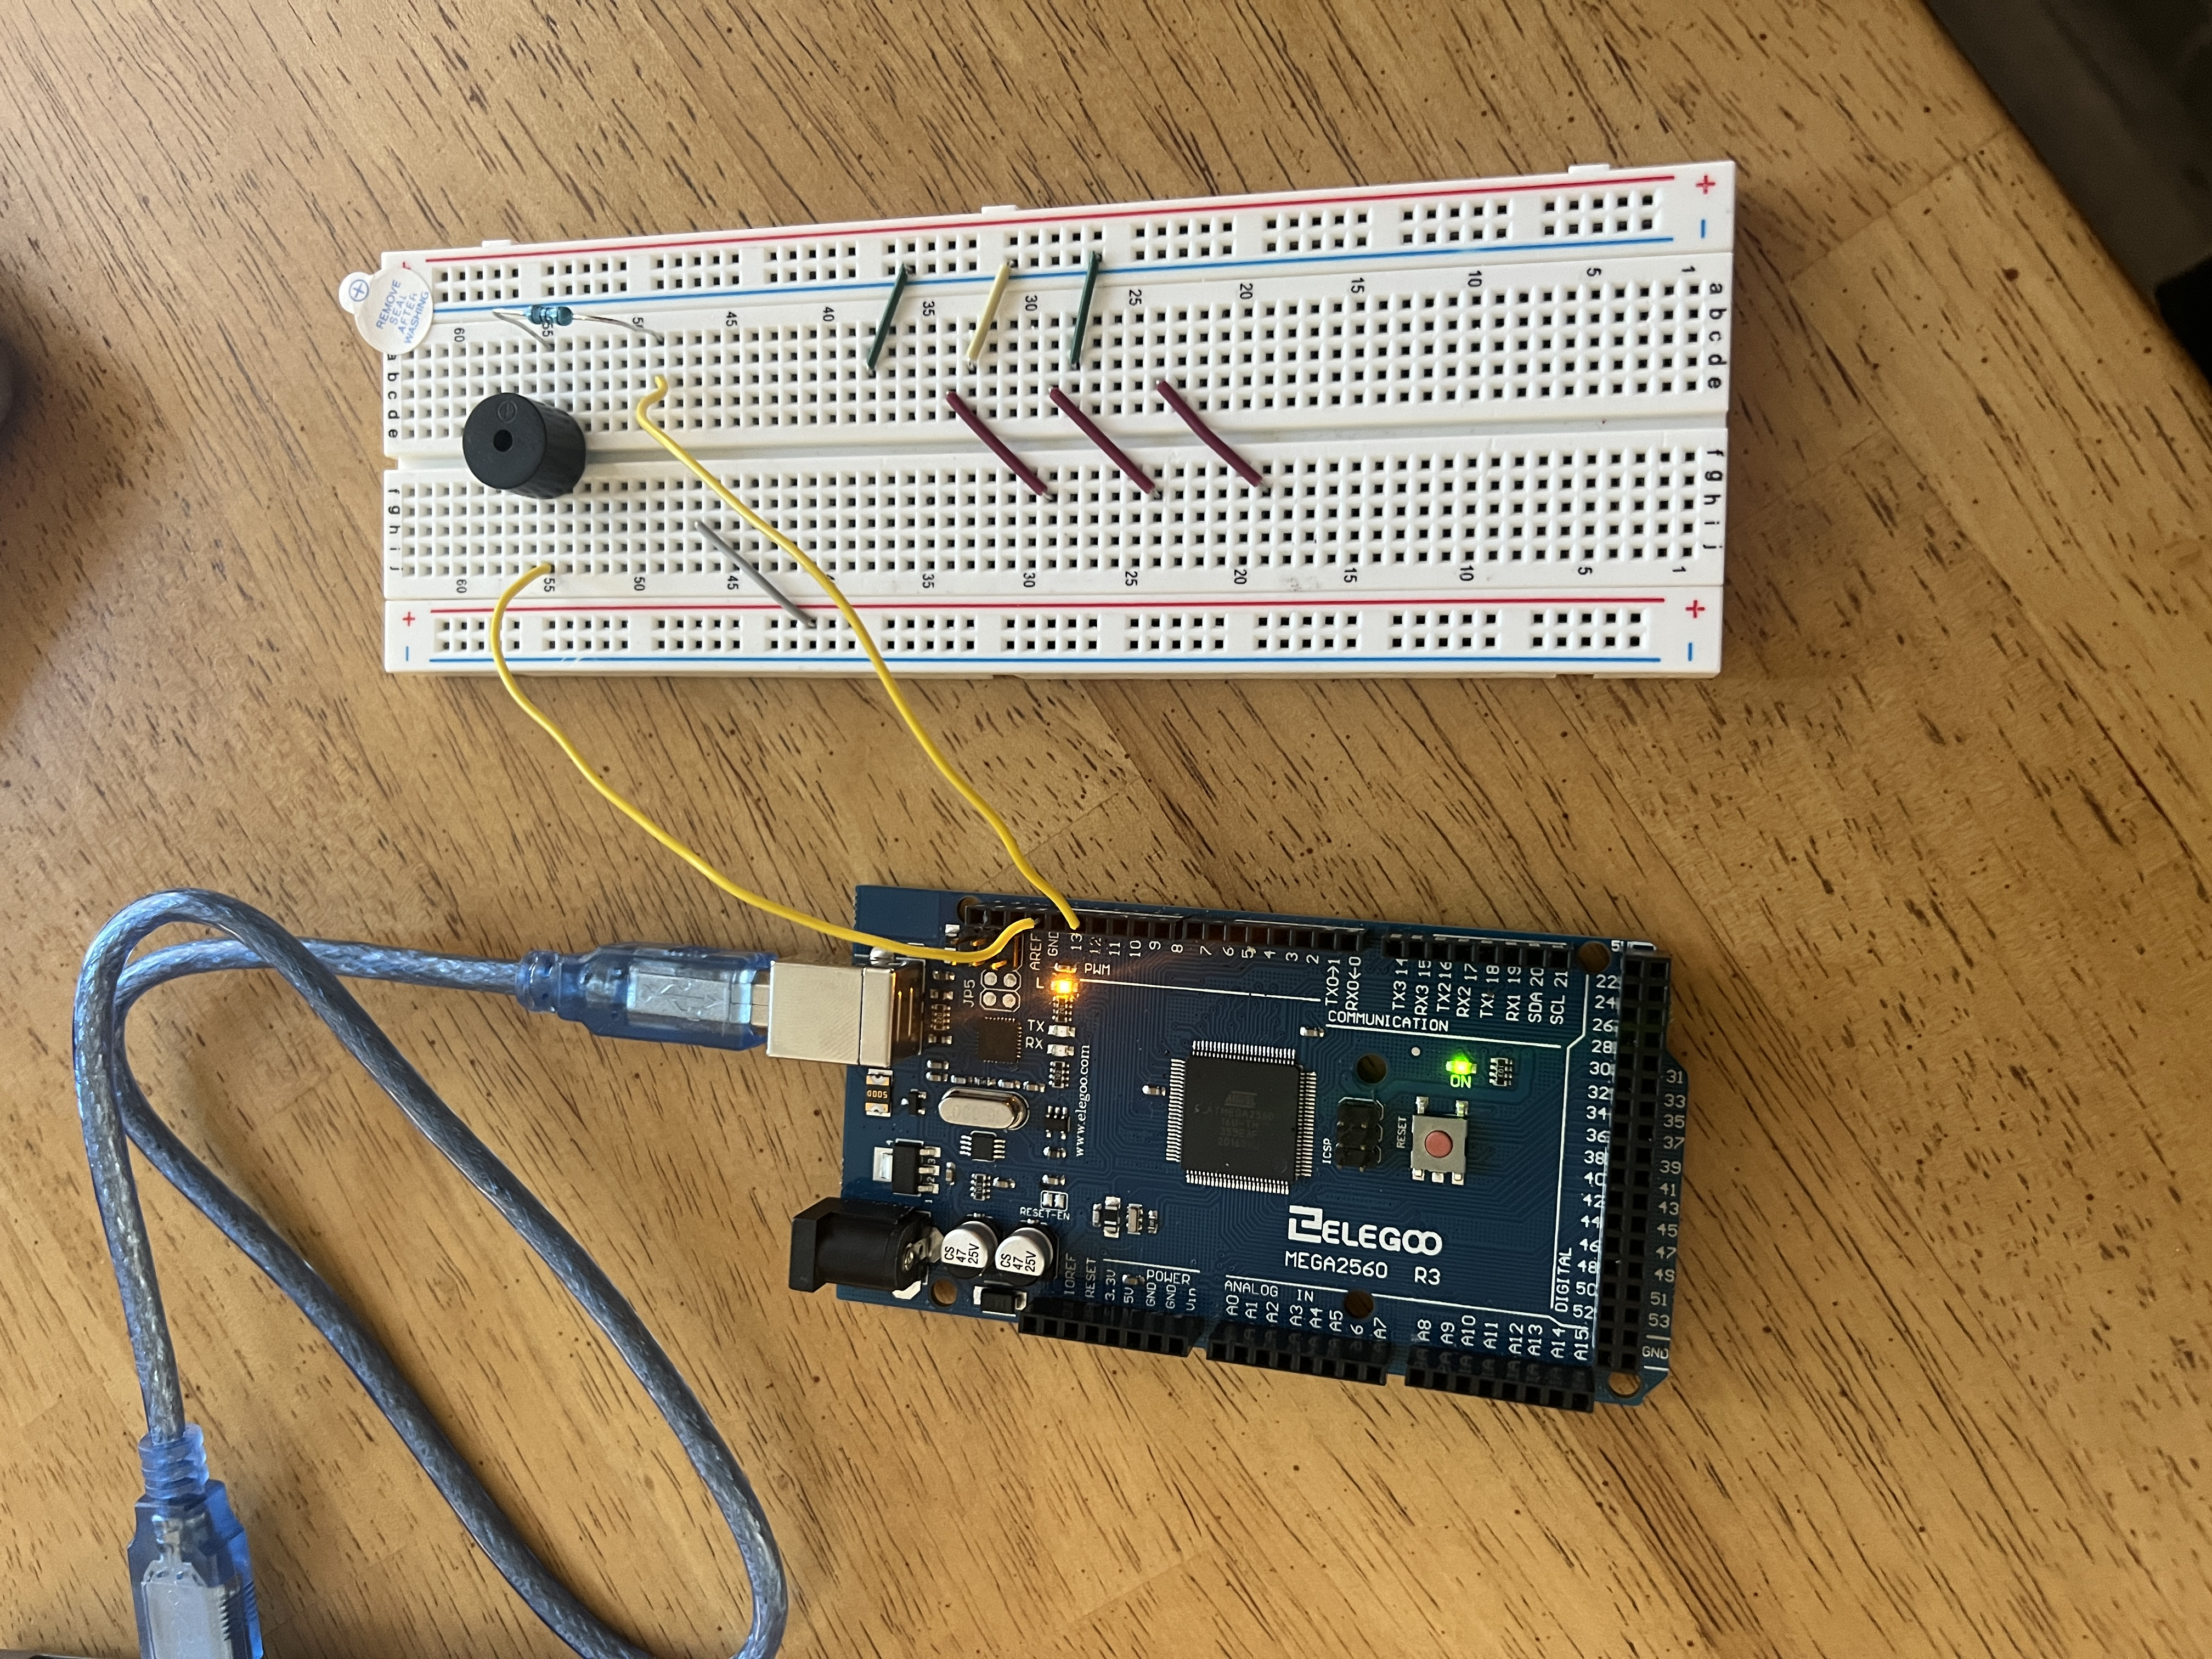
\includegraphics[width=0.5\textwidth]{circuit.JPG}
\caption{\label{fig:circuit}The buzzer circuit, wired through a 100 $\Omega$ resistor.}
\end{figure}

\subsection{Code}


The program listens for keyboard inputs from the serial monitor and plays musical notes (A–G see Table \ref{tab:frequencies}) on pin PB6 (Arduino Mega pin 12) by generating square waves at the corresponding frequencies. When a note key (A–G) is entered, the program calculates the appropriate timer delay using Timer1 and toggles the PB6 pin to create the tone. The sound continues until a new key is pressed, allowing continuous note playback. Pressing ‘q’ stops the tone completely by halting the timer and clearing the output pin.

The function my\_delay() uses direct register manipulation to configure Timer1 in normal mode. It computes how many timer ticks are needed for half of the waveform period, preloads the counter to overflow after that time, and waits for the overflow flag before toggling the output pin.

\begin{table}[ht]
\begin{center}
\caption{\textit{Frequencies Corresponding to Each Keyboard Key}}
\label{tab:frequencies}
\begin{tabular}{cc}
    \hline
    \textbf{Keyboard Key} & \textbf{Note Frequency (Hz)} \\
    \hline
    A & 440 \\
    B & 494 \\
    C & 523 \\
    D & 587 \\
    E & 659 \\
    F & 698 \\
    G & 784 \\
    \hline
\end{tabular}
\end{center}
\end{table}

 
View the code on \href{https://github.com/jrkre/cpe-301}{GitHub}!

\end{document}